\documentclass[14pt]{extbook}
\usepackage{multicol, enumerate, enumitem, hyperref, color, soul, setspace, parskip, fancyhdr} %General Packages
\usepackage{amssymb, amsthm, amsmath, bbm, latexsym, units, mathtools} %Math Packages
\everymath{\displaystyle} %All math in Display Style
% Packages with additional options
\usepackage[headsep=0.5cm,headheight=12pt, left=1 in,right= 1 in,top= 1 in,bottom= 1 in]{geometry}
\usepackage[usenames,dvipsnames]{xcolor}
\usepackage{dashrule}  % Package to use the command below to create lines between items
\newcommand{\litem}[1]{\item#1\hspace*{-1cm}\rule{\textwidth}{0.4pt}}
\pagestyle{fancy}
\lhead{Progress Quiz 4}
\chead{}
\rhead{Version B}
\lfoot{4378-7085}
\cfoot{}
\rfoot{Fall 2020}
\begin{document}

\begin{enumerate}
\litem{
Determine the domain of the function below.\[ f(x) = \frac{5}{30x^{2} +10 x -20} \]\begin{enumerate}[label=\Alph*.]
\item \( \text{All Real numbers except } x = a, \text{ where } a \in [-1.2, 0.2] \)
\item \( \text{All Real numbers except } x = a \text{ and } x = b, \text{ where } a \in [-1.2, 0.2] \text{ and } b \in [-0.6, 1.1] \)
\item \( \text{All Real numbers except } x = a \text{ and } x = b, \text{ where } a \in [-25.3, -23.6] \text{ and } b \in [22.9, 24.3] \)
\item \( \text{All Real numbers except } x = a, \text{ where } a \in [-25.3, -23.6] \)
\item \( \text{All Real numbers.} \)

\end{enumerate} }
\litem{
Determine the domain of the function below.\[ f(x) = \frac{4}{15x^{2} -43 x + 30} \]\begin{enumerate}[label=\Alph*.]
\item \( \text{All Real numbers.} \)
\item \( \text{All Real numbers except } x = a \text{ and } x = b, \text{ where } a \in [0.77, 1.29] \text{ and } b \in [1.65, 1.95] \)
\item \( \text{All Real numbers except } x = a, \text{ where } a \in [14.66, 15.62] \)
\item \( \text{All Real numbers except } x = a, \text{ where } a \in [0.77, 1.29] \)
\item \( \text{All Real numbers except } x = a \text{ and } x = b, \text{ where } a \in [14.66, 15.62] \text{ and } b \in [29.92, 30.14] \)

\end{enumerate} }
\litem{
Choose the equation of the function graphed below.
\begin{center}
    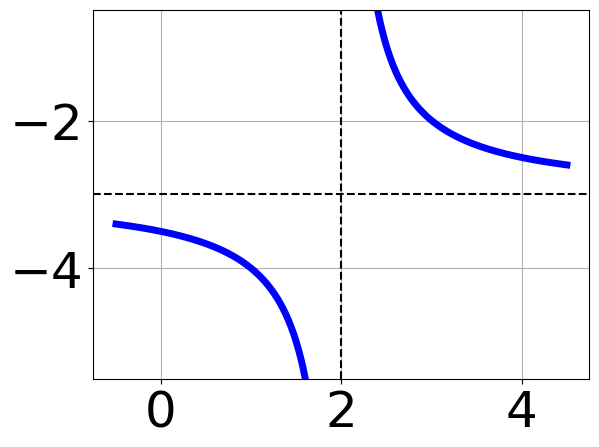
\includegraphics[width=0.5\textwidth]{../Figures/rationalGraphToEquationCopyB.png}
\end{center}
\begin{enumerate}[label=\Alph*.]
\item \( f(x) = \frac{1}{(x - 3)^2} + 1 \)
\item \( f(x) = \frac{1}{x - 3} + 1 \)
\item \( f(x) = \frac{-1}{x + 3} + 1 \)
\item \( f(x) = \frac{-1}{(x + 3)^2} + 1 \)
\item \( \text{None of the above} \)

\end{enumerate} }
\litem{
Solve the rational equation below. Then, choose the interval(s) that the solution(s) belongs to.\[ \frac{-5x}{2x + 5} + \frac{-6x^{2}}{4x^{2} -4 x -35} = \frac{-3}{2x -7} \]\begin{enumerate}[label=\Alph*.]
\item \( x_1 \in [-1.13, -0.11] \text{ and } x_2 \in [-2.11,3.89] \)
\item \( x_1 \in [-1.13, -0.11] \text{ and } x_2 \in [-2.5,-1.5] \)
\item \( x \in [3.11,3.91] \)
\item \( \text{All solutions lead to invalid or complex values in the equation.} \)
\item \( x \in [2.58,3.27] \)

\end{enumerate} }
\litem{
Solve the rational equation below. Then, choose the interval(s) that the solution(s) belongs to.\[ \frac{-48}{48x + 96} + 1 = \frac{-48}{48x + 96} \]\begin{enumerate}[label=\Alph*.]
\item \( x \in [-2.0,-1.0] \)
\item \( x_1 \in [-2, 0] \text{ and } x_2 \in [-3,0] \)
\item \( x \in [2,5] \)
\item \( x_1 \in [-2, 0] \text{ and } x_2 \in [1,3] \)
\item \( \text{All solutions lead to invalid or complex values in the equation.} \)

\end{enumerate} }
\litem{
Choose the graph of the equation below.\[ f(x) = \frac{-1}{(x - 2)^2} + 2 \]\begin{enumerate}[label=\Alph*.]
\begin{multicols}{2}\item 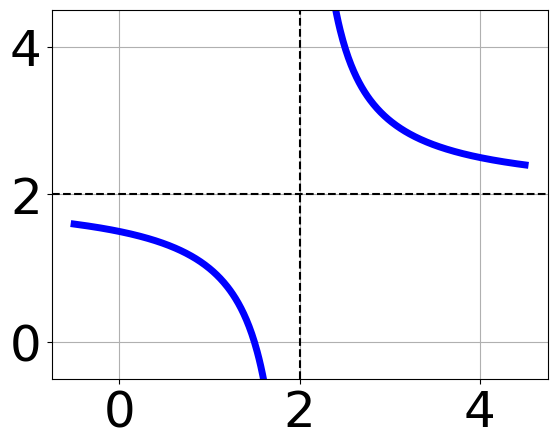
\includegraphics[width = 0.3\textwidth]{../Figures/rationalEquationToGraphAB.png}\item 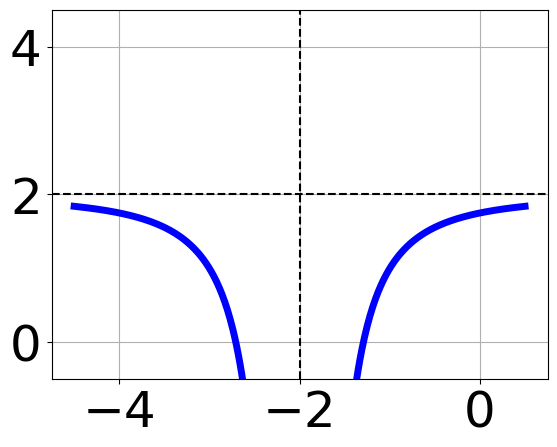
\includegraphics[width = 0.3\textwidth]{../Figures/rationalEquationToGraphBB.png}\item 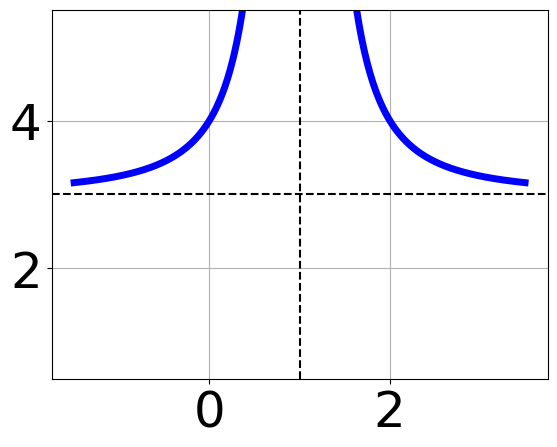
\includegraphics[width = 0.3\textwidth]{../Figures/rationalEquationToGraphCB.png}\item 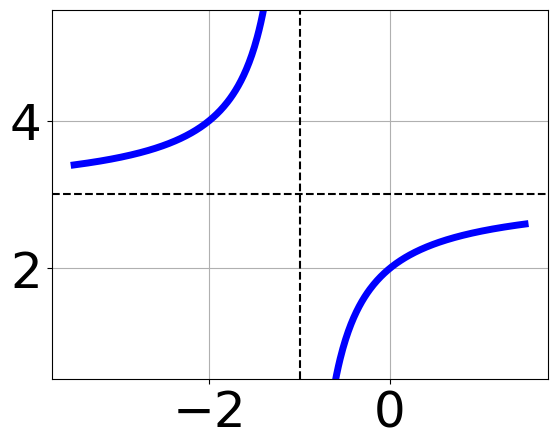
\includegraphics[width = 0.3\textwidth]{../Figures/rationalEquationToGraphDB.png}\end{multicols}\item None of the above.
\end{enumerate} }
\litem{
Choose the equation of the function graphed below.
\begin{center}
    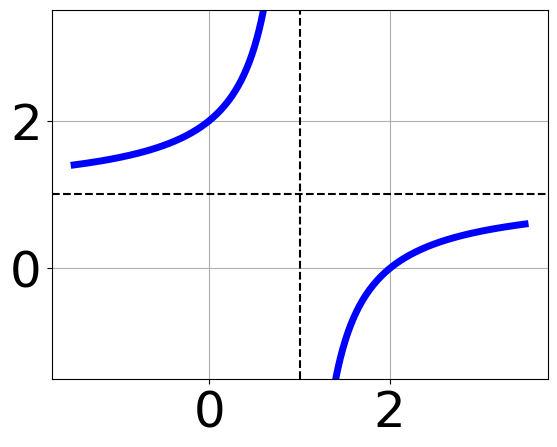
\includegraphics[width=0.5\textwidth]{../Figures/rationalGraphToEquationB.png}
\end{center}
\begin{enumerate}[label=\Alph*.]
\item \( f(x) = \frac{-1}{(x - 1)^2} + 1 \)
\item \( f(x) = \frac{1}{(x + 1)^2} + 1 \)
\item \( f(x) = \frac{-1}{x - 1} + 1 \)
\item \( f(x) = \frac{1}{x + 1} + 1 \)
\item \( \text{None of the above} \)

\end{enumerate} }
\litem{
Solve the rational equation below. Then, choose the interval(s) that the solution(s) belongs to.\[ \frac{-3x}{-7x + 7} + \frac{-2x^{2}}{-42x^{2} +77 x -35} = \frac{7}{6x -5} \]\begin{enumerate}[label=\Alph*.]
\item \( \text{All solutions lead to invalid or complex values in the equation.} \)
\item \( x \in [1.6,2.09] \)
\item \( x_1 \in [1.02, 1.36] \text{ and } x_2 \in [-0.7,1.8] \)
\item \( x_1 \in [1.02, 1.36] \text{ and } x_2 \in [1.6,2] \)
\item \( x \in [0.72,0.94] \)

\end{enumerate} }
\litem{
Solve the rational equation below. Then, choose the interval(s) that the solution(s) belongs to.\[ \frac{4}{-7x -9} + -7 = \frac{-5}{-63x -81} \]\begin{enumerate}[label=\Alph*.]
\item \( x \in [-1.38,0.62] \)
\item \( x \in [1.13,1.22] \)
\item \( x_1 \in [-1.49, -1.38] \text{ and } x_2 \in [-2.38,0.62] \)
\item \( x_1 \in [-1.39, -1.28] \text{ and } x_2 \in [0.19,4.19] \)
\item \( \text{All solutions lead to invalid or complex values in the equation.} \)

\end{enumerate} }
\litem{
Choose the graph of the equation below.\[ f(x) = \frac{1}{(x + 3)^2} + 3 \]\begin{enumerate}[label=\Alph*.]
\begin{multicols}{2}\item 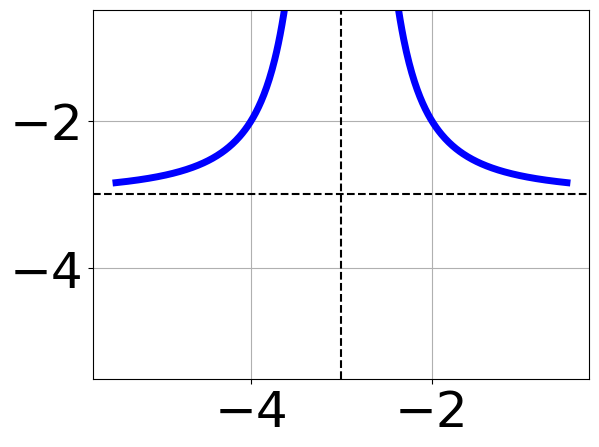
\includegraphics[width = 0.3\textwidth]{../Figures/rationalEquationToGraphCopyAB.png}\item 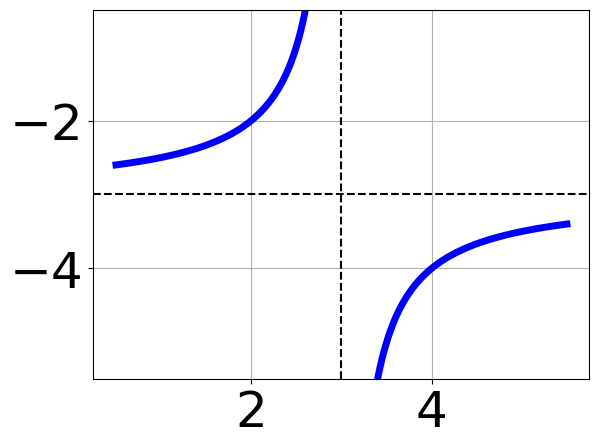
\includegraphics[width = 0.3\textwidth]{../Figures/rationalEquationToGraphCopyBB.png}\item 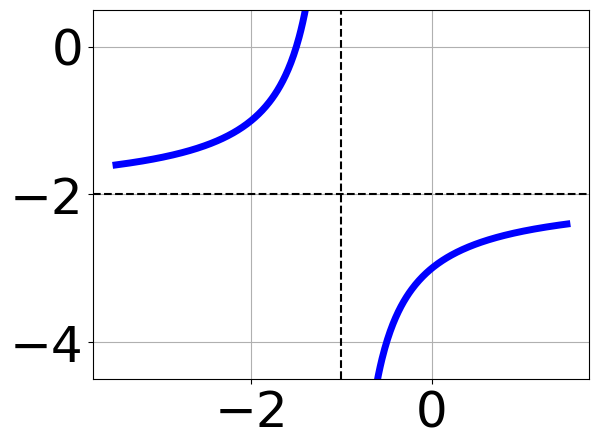
\includegraphics[width = 0.3\textwidth]{../Figures/rationalEquationToGraphCopyCB.png}\item 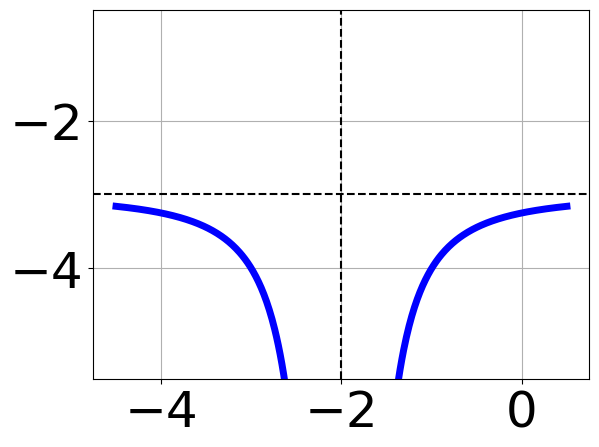
\includegraphics[width = 0.3\textwidth]{../Figures/rationalEquationToGraphCopyDB.png}\end{multicols}\item None of the above.
\end{enumerate} }
\end{enumerate}

\end{document}